% !TeX spellcheck = en_US
\documentclass[a4paper,fleqn,11pt]{article}

%% Packages 

% Styling TOC
\usepackage{tocloft}
\setlength\cftaftertoctitleskip{1cm}
\usepackage[nottoc]{tocbibind}

% Mathe Packages
\usepackage{amsmath,amssymb,epsfig,amsthm,amsfonts,bbm,textcomp}
\usepackage{blkarray}
\newcommand{\matindex}[1]{\mbox{\scriptsize#1}}% Matrix index

% Grafiken
\usepackage[font=small,aboveskip=0pt,belowskip=0pt,labelfont=bf,textfont=bf]{caption}
\captionsetup{justification=justified,singlelinecheck=false}
\captionsetup[table]{labelsep=period}
\def\captionab#1#2{\caption[#1]{#1. \normalfont\small{#2}}}
\usepackage[section]{placeins}

% Schrift
\usepackage[utf8]{inputenc}
\usepackage[T1]{fontenc}
\usepackage{lmodern}
\usepackage[english]{babel}

% Seiten Layout
\usepackage{float} 				
%\usepackage[top=3cm,bottom=3cm,left=3cm,right=3cm,a4paper]{geometry}    
%\usepackage[onehalfspacing]{setspace}
\usepackage[top=2.5cm,bottom=2.5cm,left=2.5cm,right=2.5cm,a4paper]{geometry}
%\usepackage[doublespacing]{setspace}
\usepackage{color}
\usepackage{enumitem}
\usepackage{authblk}
\setlength{\parindent}{0pt}
\usepackage{pdflscape}

% Fussnoten
\usepackage[flushmargin,hang]{footmisc}
\usepackage{listings}
\usepackage[hidelinks]{hyperref}
\usepackage{url}

% Tabellen
\usepackage{longtable} 			% Lange, mehrseitige Tabelle
\usepackage{tabularx}
\usepackage{array,hhline}
\usepackage{booktabs}			% Linien zwischen Zeilen 
\usepackage{multirow}			% Verknüpfte Zellen über Zeilen hinweg
\usepackage{dcolumn}			% Erlaubt variable Orientierung am Decimalpunkt innerhalb einer Zelle
\usepackage{rotating} % Drehung von Tabellen

\usepackage{threeparttable}

% References
\usepackage{natbib}
\bibliographystyle{apa}

% Sonstiges
\usepackage[colorinlistoftodos]{todonotes}


\begin{document}

\title{\huge The Effect of Improved Maize Seeds and Fertilizers on Crop Yields \\
\LARGE Assignment: Identification and Causal Inference}

\author{Jonas Schmitt, Sina Streicher, Owen Cortner, Philipp Kronenberg}

\date{\small \today}

\clearpage\maketitle
\thispagestyle{empty}

\renewcommand{\labelenumi}{\alph{enumi})}

\section{Introduction} \label{sec:introduction}

We examine the effect of a package of improved maize seeds and fertilizers on the harvested amount of maize of small-scale agricultural households. Maize is an important source of carbohydrates in the imaginary country, which we examine. The result of the study should evaluate if the package is manageable and effective with a limited amount of extension service and if it can help to improve the food self-supply situation of those households. 

The package of improved maize seeds and fertilizers can be picked up for free at several supply stations throughout the research area. Agricultural households have been informed in person by a group of young students about the process and where they can pick up the package. The information was spread by considering a federal list of all agricultural households in the study area. The total number of agricultural households in the list was 10.000. 5.000 households were randomly picked and received a voucher to pick up the seed + fertilizer package. 

However, we observe that only a subgroup of agricultural households takes the treatment by picking up the seed + fertilizer package. We guess that e.g. the distance to the supply stations of a household, the education (as read/write dummy) or number of very young children (< 10 years) influences the choice to pick up the package and that the selection of treatment is therefore not random. 

Unfortunately, we have no information about the soil quality, which has an influence on the amount harvested even without any treatment. Therefore, we also face the issue of omitted variable bias. 

\begin{enumerate}
\item Experiment

In the experiment, we would randomly distribute the package of improved seeds + fertilizers to a treatment group of agricultural households e.g. by an address-list and measure the causal effect by comparing the harvested amount between treated and untreated households. The treated households additionally receive a voucher for farm equipment after the harvest, if they apply the package to their best of knowledge and without sharing it with their neighbours or any family members. Thereby, we want to avoid any spill-over effects between treatment and control group.

\item Optimal Data Set

The optimal dataset would reveal all the relevant variables from an agricultural perspective (soil quality, topographic information, weather data on each farm etc.) and socioeconomic variables like income situation, education or family composition.

\item Threats to Identification

The issue of omitted variable bias is the first threat to the identification strategy. It is caused by factors that determine the assignment to treatment and which are at the same
time correlated with the outcome. The second threat is the validity of the instrument. Experiments often have a great internal validity (within the context of a particular sample/study). However, it is not always clear if the results of a certain subsample have an external validity and can be generalized to other subgroups and circumstances.

\end{enumerate}

\section{Data Generation and Model Specification} \label{sec:data}

In this experiment we consider a sample consisting of 10.000 observations. Each observation represents one individual agricultural household, indicated by the subscript $\textit{i}$. The outcome variable $\textit{harv}_i$ represents the amount harvested (kg) by individual $\textit{i}$. Our treatment $\textit{D}_i \in \{0,1\}$ is a binary variable that indicates whether individual $\textit{i}$ used the package of improved maize seeds and fertilizers or not. Therefore, $\textit{D}_i = 1$ means that the individual received the treatment and $\textit{D}_i = 0$ means no treatment. To control for other relevant variables, we collected the following covariates: $\textit{area}_i$ is the cultivated area with maize by farmer ($m^2$), which is uniformely distributed between 100 and 5000 square meters. $\textit{sun}_i$ is the sun-hours during growing period (h), which is uniformly distributed between 400 and 600 hours. $\textit{rain}_i$ is the total rainfall during growing period (mm), which is uniformly distributed between 600 and 850 millimetres. $\textit{child}_i$ is the number of children under 10 years, which is uniformly distributed between 0 and 5. $\textit{exp}_i$ is the years of experience and is uniformly distributed between 1 and 35 years. $\textit{educ}_i$ is a binary variable indicating whether individual \textit{i} is able to write and read ($\textit{educ}_i = 1$) or not ($\textit{educ}_i = 0$). In this study, we assume that the variable $\textit{educ}_i$ is unobserved.

%I excluded income since it would lead to an endogeneity problem?!
%Could also include married or partner/single and interaction term with children


%Cultivated area with maize (m2): $\textit{area}_i \sim$ U(100, 5000) \\
%Sun-hours during growing period (h): $\textit{sun}_i \sim$ U(400, 600) \\
%total rainfall during growing period (mm): $\textit{rain}_i \sim$ U(600, 850) \\
%Number of children under 10 years: $\textit{child}_i \sim$ U(0, 5)  \\
%Years of experiences: $\textit{exp}_i \sim$ U(1, 35) \\
%Education: $\textit{educ}_i \sim$ U\{0,1\}, where 1 is good and 0 bad reading and writing skills \\
%Distance to the supply stations of a household (km): $\textit{dist}_i \sim$ U(1, 100) \\

In the following analysis we want to estimate the causal effect of the treatment on the outcome variable as described in the following equation: 
\begin{align}
	\label{eq:eq1}
	\textit{Y}_i &= \boldsymbol{\mu}(0) + \boldsymbol{\Delta}_i \textit{D}_i + \textit{U}_i(0),
\end{align}
where $\textit{Y}_i$ is the outcome by individual, $\boldsymbol{\mu}(0) = \textit{Y}_i(0)$ is the outcome by individual without treatment and $\boldsymbol{\Delta}_i$ is the causal effect of the treatment  for individual \textit{i}.
\begin{equation}
  \begin{aligned}
	\label{eq:eq2}
	\boldsymbol{\Delta}_i &= \textit{Y}_i(1) - \textit{Y}_i(0) \\
						 &= [\boldsymbol{\mu}(1)- \boldsymbol{\mu}(0)] + [\textit{U}_i(1)-\textit{U}_i(0)] \\
						 &= \boldsymbol{E} \{ \boldsymbol{\Delta}_i \} + [\textit{U}_i(1)-\textit{U}_i(0)],
  \end{aligned}
\end{equation}
represents the causal effect of treatment for individual \textit{i}, which is composed of the common gain and the idiosyncratic gain. As indicated by \cite{imbens2015causal}, these potential outcomes by individual \textit{i} according to treatment can only be interpreted as causal effect, if the assignment between treatment and no treatment is random and there arises no selection bias such that we can compare outcomes of treated and untreated individuals with same characteristics as unobserved counterfactual. If we use this model in a regression, we receive the following causal equation
\begin{equation}
  \begin{aligned}
	\label{eq:eq3}
	\textit{Y}_i &= \boldsymbol{\mu}(0) + \boldsymbol{E} \{ \boldsymbol{\Delta}_i \} \textit{D}_i + \textit{U}_i(0) + \boldsymbol{\Delta}_i[\textit{U}_i(1)-\textit{U}_i(0)] \\
				 &= \boldsymbol{\mu}(0) + \boldsymbol{\beta} \textit{D}_i + \boldsymbol{\epsilon}_i,
  \end{aligned}
\end{equation}
which only holds if $\boldsymbol{E}\{\textit{D}_i\boldsymbol{\epsilon}_i\} \neq 0$, therefore we do not have exogeneity. Assuming we could observe all relevant covariates, our regression of the true model would look the following
\begin{align}
	\label{eq:eq4}
	\textit{harv}_i &= 400 + 0.05 \textit{area}_i + 0.04 \textit{sun}_i + 0.03 \textit{rain}_i - 5 \textit{child}_i + 5 \textit{exp}_i + 10 \textit{educ}_i + 100 \textit{D}_i + \textit{e}_i,
\end{align}
where $\textit{e}_i \sim \mathcal{N}(0,\,1)$. The coefficients are chosen such that the data generated is reasonable in a stylized real life scenario. 


\section{Assignment into Treatment} \label{sec:assignment}

\begin{enumerate}
\item Two different assignments into treatment

Keeping the idiosyncratic treatment effect $\boldsymbol{\Delta}_i$ fixed, the assignment of individuals into treatment can play a major role in causal inference. Therefore, we need to discuss different cases. In the optimal case we would like to observe a random assignment into treatment. In that case we would observe that characteristics of treated and untreated individuals are balanced. The equation would look like following:
\begin{align}
	\label{eq:eq5}
	\textit{D}_i^\ast \sim U(-1, 1), 
	\qquad \text{and}  \qquad
 	\textit{D}_i =
    	\begin{cases}
      1 & \text{if $\textit{D}_i^\ast \geq$ 0}\\
      0 & \text{if $\textit{D}_i^\ast <$ 0}
    	\end{cases}. 
\end{align}
However, there are several reason, why the assignment into treatment could be not random. For example, we expect that the distance to the supply stations of a household decreases the probability to take the treatment. Education (can read/write) is supposed to have an influence on farmers evaluation regarding the effectiveness / advantage of improved seeds + fertilizer package. Thus, a better education (as read/write dummy) would increase the probability to take the treatment. In this study, we assume that $\textit{educ}_i$ is unobserved. Furthermore, the number of very young children (< 10 years) decreases the possibility to pick up the package and therefore decreases the probability to take the treatment. Therefore, the selection of treatment is not random. This leads to unbalanced characteristics of treated and untreated individuals. The data generation in the self-selection case can be described as followed:
%\begin{align}
%	\label{eq:eq8}
%	\textit{D}_i^\ast &= \boldsymbol{\gamma}_0 - \boldsymbol{\gamma}_1 \textit{dist}_i + \boldsymbol{\gamma}_2 \textit{educ}_i -  \boldsymbol{\gamma}_3 \textit{child}_i + \boldsymbol{\gamma}_4 \textit{exp}_i  + \textit{u}_i.
%\end{align}
\begin{align}
	\label{eq:eq6}
	\textit{D}_i^\ast &= 1 - 0.02 \textit{dist}_i + 2 \textit{educ}_i -  0.4 \textit{child}_i + \textit{u}_i 
	\qquad \text{and}  \qquad  
	\textit{D}_i =
    \begin{cases}
      1 & \text{if $\textit{D}_i^\ast \geq$ 0}\\
      0 & \text{if $\textit{D}_i^\ast <$ 0}
    \end{cases}. 
\end{align}

\item Descriptive statistics of raw data

In the following table the mean values of the outcome and the covariates of the simulated raw data are illustrated by treatment status (treated and untreated) and assignment mechanism (random and self-selection). %Statistical test! Report p-values!

\begin{table}[h!]
\centering
\begin{threeparttable}
\caption{Summary Statistics} \label{tab:data}
\begin{tabular}{lrrrrrrr}
  \hline
  & &\multicolumn{3}{c}{Random Assignment} & \multicolumn{3}{c}{Self-Selection}\\
 & Total & Treatment & No Treatment & P-Value & Treatment & No Treatment & P-Value\\
 \hline
harv & 677.25 & 752.78 & 651.75 &  & 978.75 & 624.12 &  \\ 
  area & 2549.94 & 2544.39 & 2551.82 & 0.82 & 2481.00 & 2566.55 & 0.02 \\ 
  sun & 500.04 & 499.41 & 500.25 & 0.53 & 501.51 & 499.68 & 0.22 \\ 
  rain & 725.10 & 725.33 & 725.02 & 0.85 & 724.28 & 725.30 & 0.58 \\ 
  exp & 17.90 & 18.10 & 17.84 & 0.24 & 17.99 & 17.88 & 0.67 \\ 
  dist & 50.59 & 51.51 & 50.28 & 0.06 & 39.25 & 53.32 & 0.00 \\ 
  child & 2.50 & 2.52 & 2.50 & 0.54 & 1.92 & 2.64 & 0.00 \\ 
  educ & 0.50 & 0.51 & 0.49 & 0.08 & 0.94 & 0.39 & 0.00 \\ 
  Obs & 10000 & 2524 & 7476 &  & 1941 & 8059 &  \\ 
   \hline
\end{tabular}
\end{threeparttable}
\footnotesize{Notes: In the table are the mean values of the variables for the different assignment and treatment groups. \textit{Obs} denotes the number of observations. P-Values are calculated with an unpaired two-samples t-test.}
\end{table}

If treatment was randomly assigned, there is no significant difference in the mean of the covariates for the treated and untreated sample. Thus, a random assignment would allow us to identify the causal treatment effect by calculating the differences in the mean for the outcome variable between treated and untreated sample. Taking a look at the p-values of the  unpaired two-samples t-test, we can see that the means of the covariates are mostly not significantly different from each other. However, in the self-selection case, we see that the variables $\textit{child}_i$, $\textit{educ}_i$, and $\textit{dist}_i$ are not balanced between treated and untreated sample and the p-values show that the means for those variables are highly significantly different from each other. Since these variables have an effect on the outcome variable $\textit{harv}_i$, the distribution of the outcome variable looks different as we can observe in the density plots.

\begin{figure}[htb]
\begin{raggedleft}
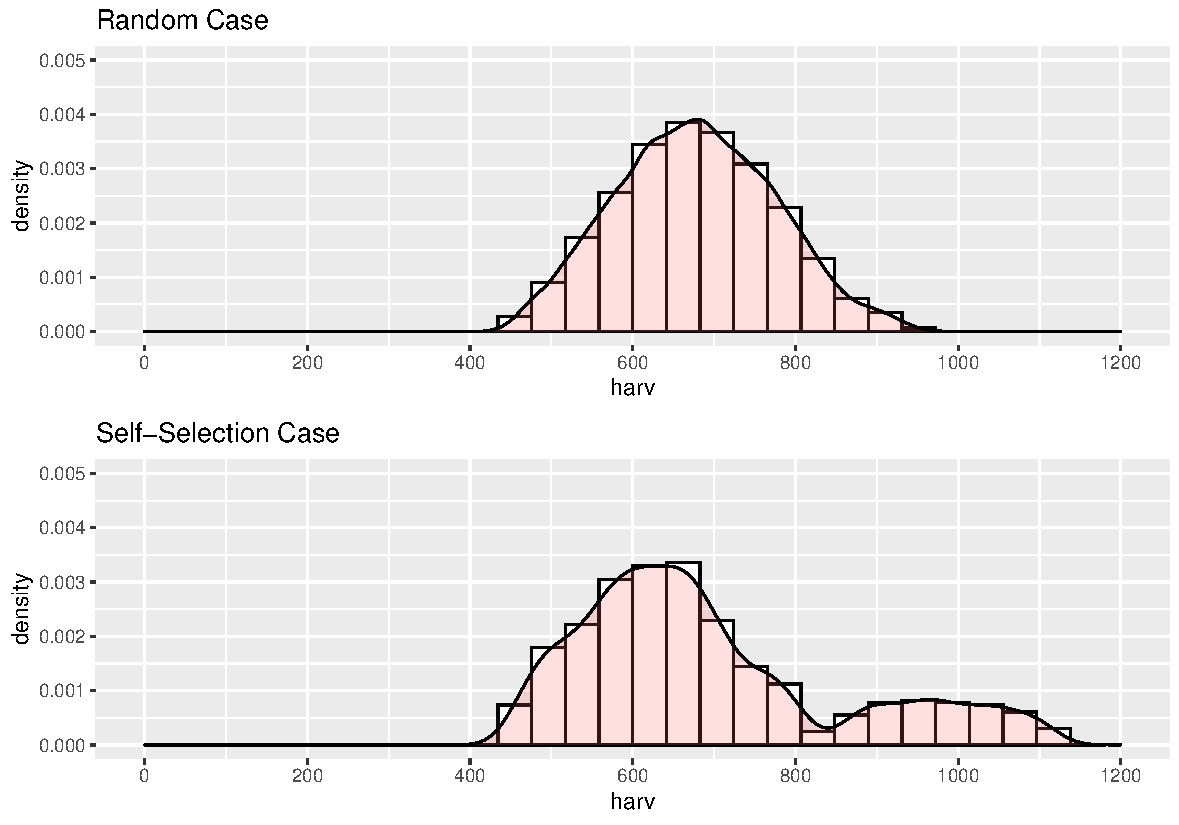
\includegraphics[width=\linewidth]{../figures/density_total.pdf}
\caption{Density function}
\label{fig:density}
\footnotesize{Notes: Density function of the variable \textit{harv} for the two assignments.}
\end{raggedleft}
\end{figure}

\begin{figure}[htb]
\begin{raggedleft}
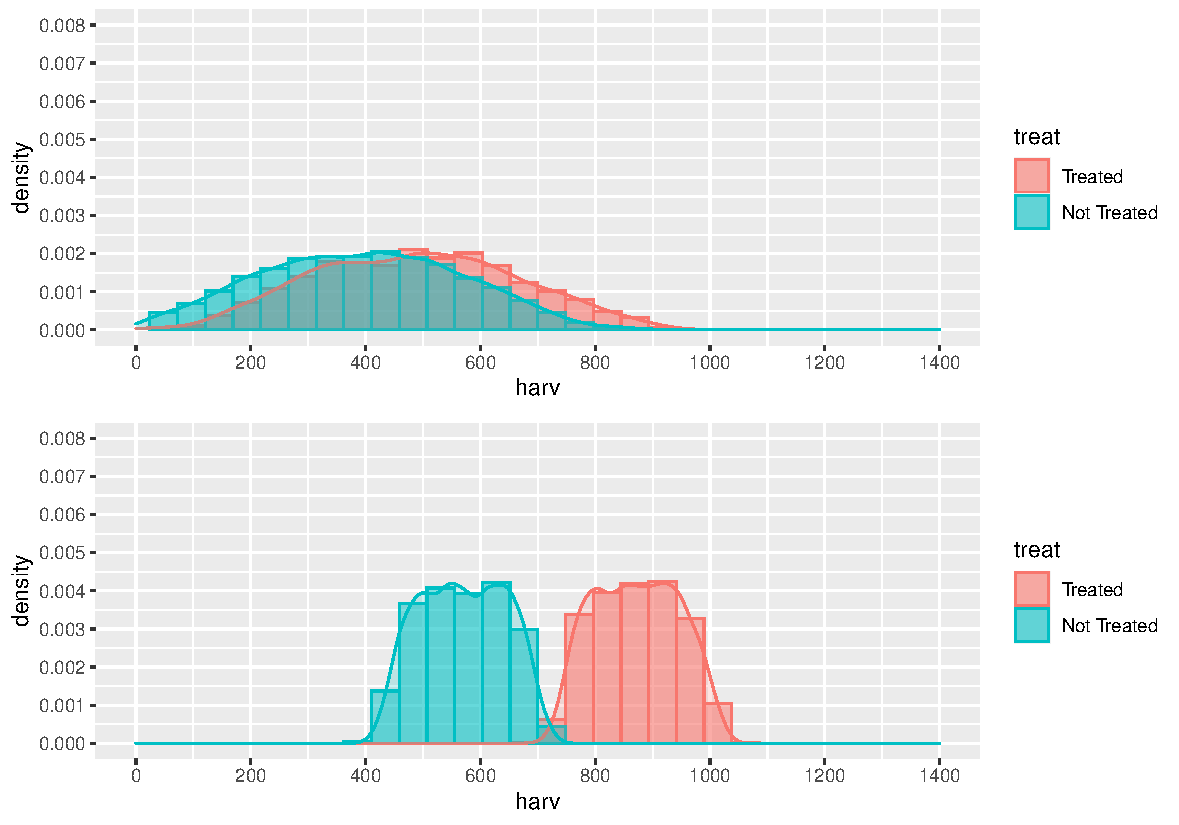
\includegraphics[width=\linewidth]{../figures/density_goups.pdf}
\caption{Density function grouped by treatment}
\label{fig:density_groups}
\footnotesize{Notes: Density function of the variable \textit{harv} for the two assignments and treatments.}
\end{raggedleft}
\end{figure}

\item Model estimation

At this point we assume that we do not know the data generating process for the two assignment cases (random and self-selection) and we want to estimate the model for the two cases. The regression contains all the relevant covariates except for $\textit{educ}_i$, which we assume to be unobserved. For both cases, we estimate the following model:

\begin{align}
	\label{eq:eq7}
	\textit{harv}_i &= \boldsymbol{\beta}_0 + \boldsymbol{\beta}_1 \textit{area}_i + \boldsymbol{\beta}_2 \textit{sun}_i + \boldsymbol{\beta}_3 \textit{rain}_i - \boldsymbol{\beta}_4 \textit{child}_i + \boldsymbol{\beta}_5 \textit{exp}_i + \boldsymbol{\Delta}_i \textit{D}_i + \textit{e}_i.
\end{align}

\begin{table}[h!]
\centering
\begin{threeparttable}
\caption{OLS Regression Random Case} \label{tab:reg1}
\begin{tabular}{rrrrr}
  \hline
 & Estimate & Std. Error & t value & Pr({$>$}{$|$}t$|$) \\ 
  \hline
(Intercept) & 405.7869 & 0.6809 & 595.99 & 0.0000 \\ 
  area & 0.0500 & 0.0000 & 1418.31 & 0.0000 \\ 
  sun & 0.0412 & 0.0009 & 48.01 & 0.0000 \\ 
  rain & 0.0291 & 0.0007 & 42.07 & 0.0000 \\ 
  exp & 4.9963 & 0.0051 & 982.34 & 0.0000 \\ 
  child & -4.9508 & 0.0334 & -148.06 & 0.0000 \\ 
  treat & 100.2027 & 0.1151 & 870.66 & 0.0000 \\ 
   \hline
\end{tabular}
\end{threeparttable}
\end{table}

The regression perfectly fits the data generating process and estimates the treatment effect correctly, even though the unobsreved variable $\textit{educ}_i$ is left out, since it is balanced across the two treatment groups. In the case of the self-selection we obtain the following results:

\begin{table}[h!]
\centering
\begin{threeparttable}
\caption{OLS Regression Self-Selection Case} \label{tab:reg2}
\begin{tabular}{rrrrr}
  \hline
 & Estimate & Std. Error & t value & Pr({$>$}{$|$}t$|$) \\ 
  \hline
(Intercept) & 433.6133 & 6.0982 & 71.11 & 0.0000 \\ 
  area & 0.0499 & 0.0003 & 158.18 & 0.0000 \\ 
  sun & 0.0472 & 0.0077 & 6.14 & 0.0000 \\ 
  rain & 0.0235 & 0.0062 & 3.79 & 0.0002 \\ 
  exp & 1.4605 & 0.0455 & 32.09 & 0.0000 \\ 
  child & -1.5903 & 0.3048 & -5.22 & 0.0000 \\ 
  treat & 357.5306 & 1.1528 & 310.15 & 0.0000 \\ 
   \hline
\end{tabular}
\end{threeparttable}
\end{table}

Here, we can see a large bias. The treatment effect is estimated much larger than it is in real. This is due to the omitted variables leading to self-selection. For the variable $\textit{educ}_i$ we expect the omitted variable bias to be positive, since it is positively correlated with the treatment and the output variable. 

\end{enumerate}


% -------------------------------------------------------------------------------
\section{Selection Bias} \label{sec:selection}

However, we expect that e.g. the distance to the supply stations of a household, the education (as read/write dummy) or number of very young children (< 10 years) influences the choice to pick up the package and that the selection of treatment is therefore not random. Thus, self-selection into treatment depends on the unobserved variable education. As a result, the model suffers from omitted variable bias, since the treatment is not independent of the error term, $Cov(\textit{D}_i, \textit{e}_i) = 0$. As a result, the conditional independence assumption (CIA) is not fulfilled and a causal interpretation of the coefficients is not possible.
%Unobserved: Soil quality, topographic information OVB

For this reason, we follow an alternative instrument variable approach following 
\begin{align}
	\label{eq:eq8}
	\textit{D}_i^\ast &= \boldsymbol{\alpha} + \boldsymbol{\beta} \textit{Z}_i + \textit{V}_i.
\end{align}
As instrument variable we use a random assignment to receive a voucher to pick up the seed + fertilizer package. $\textit{vouch}_i$ is a binary variable indicating whether individual \textit{i} received a voucher ($\textit{vouch}_i = 1$) or not ($\textit{vouch}_i = 0$). This results in the equation
\begin{align}
	\label{eq:eq9}
	\textit{D}_i^\ast &= \boldsymbol{\alpha} + \boldsymbol{\beta} \textit{vouch}_i + \textit{v}_i.
\end{align}
where $\textit{v}_i \sim \mathcal{N}(0,\,1)$. This random assignment of the voucher is correlated with treatment, since we expect a positive share of individuals receiving the voucher will pick up the package and only individuals receiving the voucher are allowed to pick up the package. Furthermore, the instrument is correlated with the outcome variable, since receiving the treatment should have an effect on output. Finally, the instrument is uncorrelated with the error term $\boldsymbol{\epsilon}_i$ since the assignment of receiving the voucher is randomly picked. As a result, the following holds
\begin{align}
	\label{eq:eq10}
	\boldsymbol{E}\{\textit{U}_i(1)\} = \boldsymbol{E}\{\textit{U}_i(0)\} = \boldsymbol{E}\{\textit{V}_i(1)\} = 0.
\end{align}


% -------------------------------------------------------------------------------
\section{Difference in Difference} \label{sec:difference}


% -------------- part 5a

In a next step, we generate five repeated cross sections from 2000 until 2004 using a similar data generating process as above. For convenience, we now use $n=100$ households. The variables $area, educ,$ and $dist$ are held constant in time. For the variable $child$, we assume that each year, the number of children below the age of 10 either increases or decreases by one, each with probability $\nicefrac{1}{6}$.\footnote{An increase in the number of children below the age of 10 is associated with a newborn child. A decrease is due to children turning 10 or dying.} The variables related to weather conditions, $rain$ and $sun$ are redrawn for each year, i.e., we assume that there are no weather trends and that each households faces a similar climate. Further. we assume no harvest worker dies during the five year period, assuring that experience $exp$ grows linearly. In the beginning of 2003, the vouchers for the seed and fertilizer package are distributed and we assume that each household receiving a voucher decides whether or not to take up the offer for the ongoing and the next year.


Figure \ref{fig:did_a} shows the harvest output of the treatment and the control groups. The treatment group comprises all households that received a voucher in 2003 and subsequently took up the offer. The control group consists of all remaining households. Notably, before the start of the treatment, the mean size of the harvest is different in the two groups due to self-selection. Yet, mean harvest moves in tandem, indicating that the parallel trend assumption is fulfilled. From 2003 onward, the harvest of the treated group experiences a level shift by about 300kg. In the control group, the same time trend as before continues.

\begin{figure}[htb]
	\begin{center}
		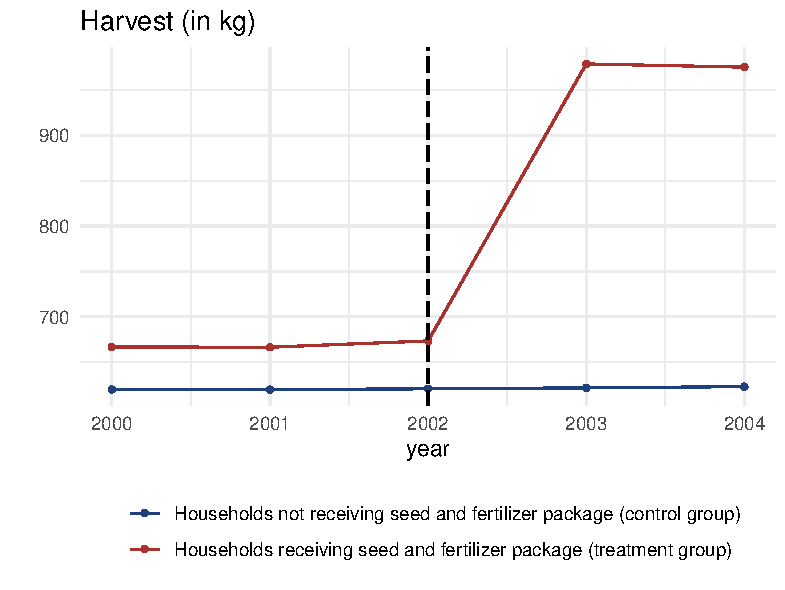
\includegraphics[width=0.55\linewidth]{../figures/part5a.pdf}
	\end{center}
%	\vspace{-1cm}
	\caption{Effect of seed and fertilizer packages on harvest.}
	\label{fig:did_a}	{\footnotesize Notes: The figure compares the harvest between the treatment and control group. The seed and fertilizer packages were distributed from 2003 onward.}
\end{figure}

% -------------- part 5b

Let $D_i$ be a time-invariant dummy that indicates whether or not a household is treated. Further, let $T_t$ be a time dummy series. By $X_{i,t}$, we denote the vector of exogenous control variables, i.e., $X_{i,t} = \left(sun_{i,t}, rain_{i,t}, child_{i,t}\right)$.\footnote{Note that the variables $area$ and $exp$ will be captured by individual and time fixed-effects and are therefore dropped here.}
We estimate the following linear model:
\begin{align}
	\label{eq:eq7did}
	harv_{i,t} &= \alpha_i + \tau_t + \delta D_{i} T_t + X_{i,t}'\beta + \epsilon_{i,t},
\end{align}
where, $\alpha_i$ and $\tau_t = \gamma T_t$ capture individual and time fixed effects. The coefficient $\delta$ captures the effect of the seed and fertilizer package on harvest. 

The results are presented in Table \ref{tab:did}. For model (1) (left column) the control variables in $X$ were omitted while model (2) (right column) includes all variables. For both models, the treatment effect roughly amounts to 300kg.

\begin{table}[!htbp] 
	\caption{Difference-in-Difference Estimation} 
	\label{tab:did} 
	\resizebox{\textwidth}{!}{\begin{tabular}{@{\extracolsep{5pt}}lcc} 
			\\[-1.8ex]\hline 
			\hline \\[-1.8ex] 
			& \multicolumn{2}{c}{\textit{Dependent variable:}} \\ 
			\cline{2-3} 
			\\[-1.8ex] & \multicolumn{2}{c}{$harv$} \\ 
			\\[-1.8ex] & (1) & (2)\\ 
			\hline \\[-1.8ex] 
			$D_i T_k$ & 300.816$^{***}$ & 300.016$^{***}$ \\ 
			& (0.941) & (0.209) \\ 
			& & \\ 
			$sun$ \textcolor{white}{spaaaaaaaaaaaaaaaaaaaaaaaaaaaaaaaaaaaaaace} &  & 0.041$^{***}$ \\ 
			&  & (0.001) \\ 
			& & \\ 
			$rain$ &  & 0.030$^{***}$ \\ 
			&  & (0.001) \\ 
			& & \\ 
			$child$ &  & $-$4.976$^{***}$ \\ 
			&  & (0.091) \\ 
			& & \\ 
			\hline \\[-1.8ex] 
			Observations & 500 & 500 \\ 
			R$^{2}$ & 1.000 & 1.000 \\ 
			Adjusted R$^{2}$ & 1.000 & 1.000 \\ 
			Residual Std. Error & 4.255 (df = 395) & 0.944 (df = 392) \\ 
			F Statistic & 117,882.900$^{***}$ (df = 105; 395) & 2,328,354.000$^{***}$ (df = 108; 392) \\ 
			\hline 
			\hline \\[-1.8ex] 
	\end{tabular} }
{\\ \footnotesize Notes: $^{*}$p$<$0.1; $^{**}$p$<$0.05; $^{***}$p$<$0.01. The estimation sample spans 2000 until 2004. The coefficient on $D_i T_k$ captures the treatment effect. The seed and fertilizer packages were distributed from 2003 onward.}

\end{table} 

% -------------- part 5c
\subsection*{Event-study difference-in-difference}

In order to explore the dynamics of the treatment effect, we extend \eqref{eq:eq7did} to estimate period-dependent treatment effects:\begin{align}
	\label{eq:eq7did_event}
	harv_{i,t} &= \alpha_i + \tau_t + \sum_{\substack{k\in  \{2000,2001, \\2003,2004\}}}\delta_k D_{i} T_k + X_{i,t}'\beta + \epsilon_{i,t}.
\end{align}
The coefficients $\delta_k$ represent the treatment effect relative to the effect in 2002. They are plotted in Figure \ref{fig:did_c}. The whiskers represent 90\% confidence intervals. As expected, prior to treatment, there is no significant effect. Once the seed and fertilizer became available to the treatment group in 2003, their harvest increased by 300kg.


\begin{figure}[htb]
	\begin{center}
		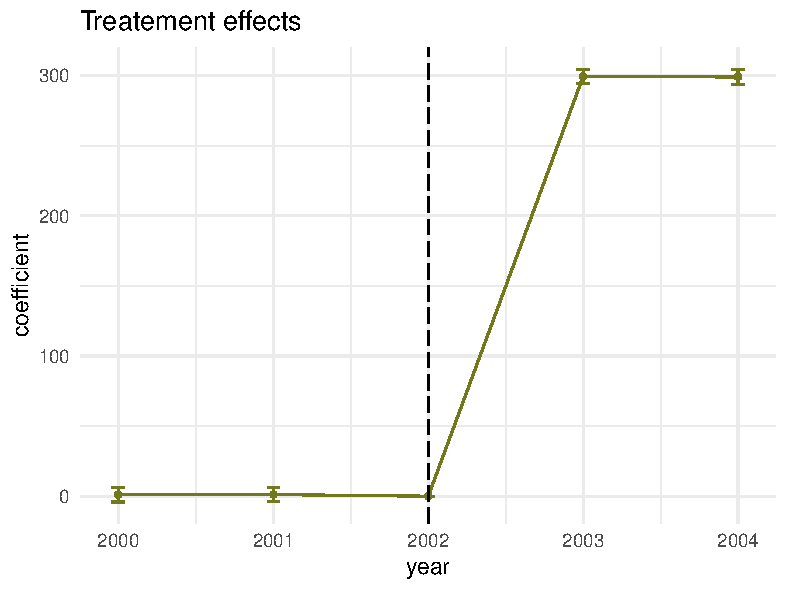
\includegraphics[width=0.55\linewidth]{../figures/part5c.pdf}
	\end{center}
	\caption{Effect of seed and fertilizer packages on harvest -- Event study.}
	\label{fig:did_c}	{\footnotesize Notes: The figure depicts the treatment effect relative to that in 2002. The whiskers represent 90\% confidence intervals. The seed and fertilizer packages were distributed from 2003 onward.}
\end{figure}


% -------------- part 5d
\subsection*{Common trend violation}

We now assume that vouchers are in fact not randomly assigned. Instead, they are distributed to those households, that are easily accessible. All households that did not receive a voucher are located in a valley in which weather conditions are more extreme. They experience both more rainfall and more sunshine and this effect intensifies over time. Unfortunately, all weather stations break down during our estimation period, which makes controlling for weather conditions impossible. 

Figure \ref{fig:did_d} shows the harvest output of the treatment and the control groups for this new set of data. 
Since sunshine and rainfall are positively associated with harvest, output in the control group shows a positive trend pre and post treatment while there are no visual differences in the treatment group prior to treatment.

\begin{figure}[htb]
	\begin{center}
		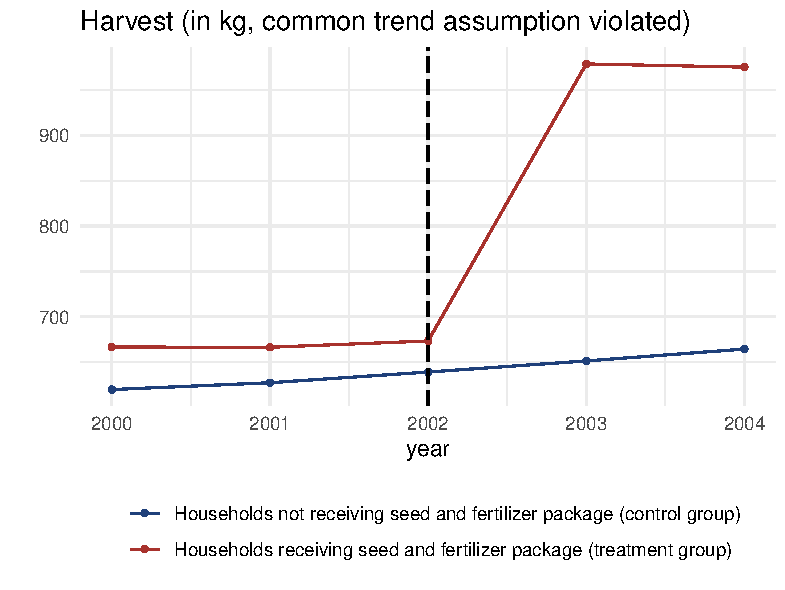
\includegraphics[width=0.55\linewidth]{../figures/part5d.pdf}
	\end{center}
	\caption{Effect of seed and fertilizer packages on harvest -- common trend violation.}
	\label{fig:did_d}	{\footnotesize Notes: The figure compares the harvest between the treatment and control group. The seed and fertilizer packages were distributed from 2003 onward.}
\end{figure}

We re-estimate \eqref{eq:eq7did_event} with the adjusted data and omit the control variables related to weather. The treatment coefficients are shown in Figure \ref{fig:did_d2}. We now observe a positive and significant treatment effect prior to 2002.


\begin{figure}[htb]
	\begin{center}
		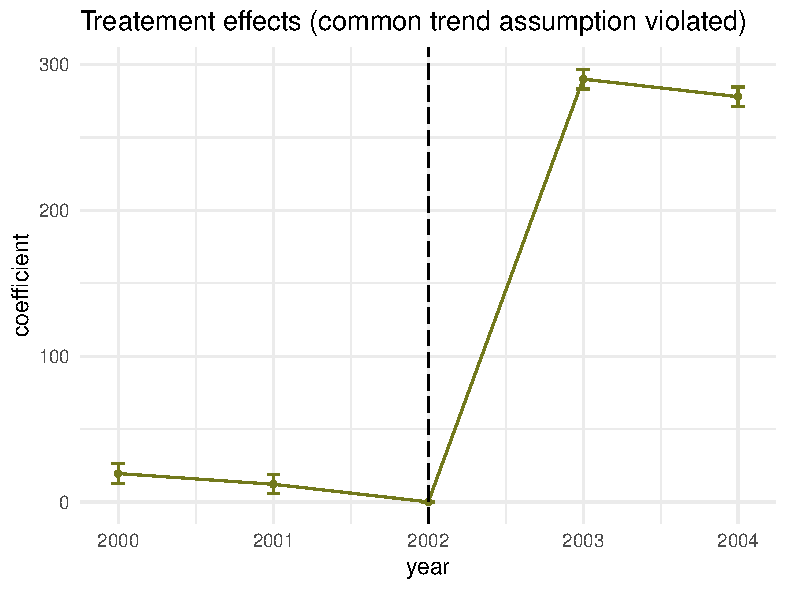
\includegraphics[width=0.55\linewidth]{../figures/part5d2.pdf}
	\end{center}
	\caption{Effect of seed and fertilizer packages on harvest -- Event study -- common trend violation.}
	\label{fig:did_d2}	{\footnotesize Notes: The figure depicts the treatment effect relative to that in 2002. The whiskers represent 90\% confidence intervals. The seed and fertilizer packages were distributed from 2003 onward.}
\end{figure}



\clearpage



\bibliography{mybibfile}

\clearpage


\end{document}